\documentclass[10pt, a4paper, ngerman]{arbeitsblatt}

\ladeModule{theme,tabellen,boxen}

\ladeFach[listings]{informatik}

\aboptionen{
	name		= {J. Neugebauer},
	kuerzel 	= {Ngb},
	titel 		= {Syntaxdiagramme},
	reihe 		= {Wiederholung der OOP},
	fach 		= {Informatik},
	kurs 		= {Q1},
	nummer 		= {I.2},
	lizenz 		= {cc-by-nc-sa-4},
	version 	= {2021-09-15},
}

\begin{document}
\ReiheTitel

\begin{infobox}
\emph{Syntaxdiagramme} stellen die Syntax einer Programmiersprache schematisch dar. Sie heißen auch Eisenbahn-Diagramm (engl. Railroad-Diagram), da sie an die Schienen einer Eisenbahn erinnern.

Man kann sie lesen, indem man sich vorstellt, ein Zug fährt vom Anfang des Diagramms immer in Pfeilrichtung durch das Diagramm. Jeder mögliche Weg, den der Zug bis zum Ende nehmen kann, stellt eine gültige Syntax in der Programmiersprache dar.
\end{infobox}

Die Syntax einer Variablen kann so definiert werden:
\begin{center}
	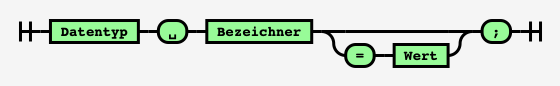
\includegraphics[width=12cm]{EF-AB.III.04-RR_Variable.png}
\end{center}

Die abgerundeten Rechtecke sind \emph{Terminale}, die genauso in den Quelltext geschrieben werden. Die Rechtecke stellen \emph{Nichtterminale} dar, die wieder durch eigene Syntaxdiagramme beschrieben werden:

\begin{multicols}{3}\centering
	\code{Bezeichner}\\
	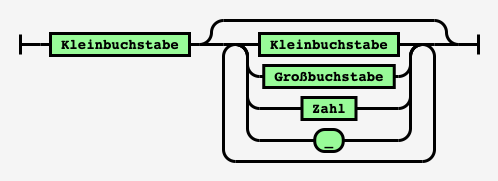
\includegraphics[width=5.5cm]{EF-AB.III.04-RR_Bezeichner.png}

	\code{Datentyp}\\
	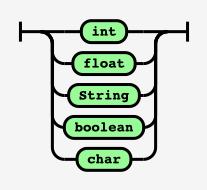
\includegraphics[width=3cm]{EF-AB.III.04-RR_Datentyp.png}

	\code{Kleinbuchstabe}\\
	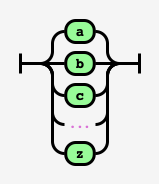
\includegraphics[width=3cm]{EF-AB.III.04-RR_Kleinbuchstabe.png}
	\columnbreak

	\code{Großbuchstabe}\\
	\includegraphics[width=3cm]{EF-AB.III.04-RR_Großbuchstabe.png}

	\code{Wert}\\
	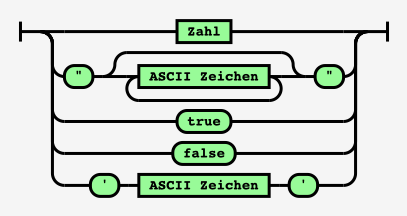
\includegraphics[width=6cm]{EF-AB.III.04-RR_Wert.png}

	\code{Zahl}\\
	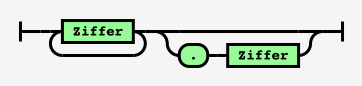
\includegraphics[width=5cm]{EF-AB.III.04-RR_Zahl.png}
	\columnbreak

	\code{Ziffer}\\
	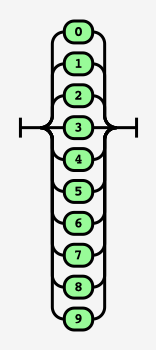
\includegraphics[width=3cm]{EF-AB.III.04-RR_Ziffer.png}
\end{multicols}

\hinweis{Klein-/Großbuchstabe wurden abgekürzt. Das Nichtterminal \code{ASCII Zeichen} wurde ausgelassen und beschreibt jedes gültige ASCII Zeichen.}

\warnung{Die Diagramme stellen nicht die vollständige Syntax von Variablendeklarationen in Java dar, sondern eine für den Unterricht vereinfachte Variante.}

\newpage

\begin{aufgabe}
Prüfe die folgenden Deklarationen, ob sie in korrekter Syntax geschrieben sind, indem du die Syntaxdiagramme oben durchgehst. Markiere \emph{alle} Fehler und überlege dir, wie sie korrigiert werden könnten.

\begin{multicols}{2}
\begin{tasks*}
	\task
	\code{int i = 1;}

	\task
	\code{float i = 000.000;}

	\task
	\code{String EinText = \scquote{Hallo}}

	\task
	\code{String 123 = \scquote{123};}

	\task
	\code{int foo = 5;}

	\task
	\code{boolean l337 = false;}

	\task
	\code{int \_foo = 5}

	\task
	\code{int \_foo = \scquote*{5};}

	\task
	\code{char einChar2Char = \scquote*{ab};}

	\task
	\code{boolean wahr\_heit;}
\end{tasks*}
\end{multicols}
\end{aufgabe}

\begin{aufgabe}
Analysiere das gezeigte Programm und erkläre seine Funktion. Gehe dabei insbesondere auf folgende Aspekte ein:
\begin{smallitem}
	\item Wozu werden hier Variablen eingesetzt?
	\item Welche Variablen sind in welchem Bereich
	\emph{gültig}?
	\item Welchen Wert haben die Variablen nach Ende des Programms?
	\item Welche neuen Befehle werden verwendet?
\end{smallitem}

\begin{lstlisting}[language=java]
int zaehler = 0;
float zahl1 = 10.0;
float zahl2 = 10.0;
char koordinate = 'A';

void setup() {
  size(255, 255);

  String name;
  name = "Alan Turing";
  println(name + " was here");

  koordinate = 'B';
}
void draw() {
  background(zaehler%256, zahl1%256, zahl2%256);

  textAlign(CENTER);
  text(koordinate, width/2, height/2);
  text(zaehler + ", " + zahl1+  ", " + zahl2, width/2, height/2+20);
}
void mouseClicked() {
  zaehler += 5;
  zahl1 = mouseX;
  zahl2 = mouseY;
  koordinate = 'C';
}
\end{lstlisting}
\end{aufgabe}

\end{document}
